\documentclass[t, aspectratio=169]{beamer}
\usepackage{amsmath,amsfonts,amsthm,amstext,amssymb, xcolor, tikz, pgf, mathrsfs, polynom, pifont, tabto}

% ----------------------------------------------------------
% Theme Setup

% Use Metropolis Theme
\usetheme[numbering=fraction]{metropolis}
\setbeamertemplate{blocks}[rounded][shadow=false]
\makeatletter
\setlength{\metropolis@titleseparator@linewidth}{1pt}
\makeatother

% Define Colors
\definecolor{chargerblue}{HTML}{002764}
\definecolor{chargerred}{HTML}{e02034}
\definecolor{bggray}{HTML}{d0d3d4}

% Set Colors
\setbeamercolor{title}{fg=chargerblue}
\setbeamercolor{background canvas}{bg=white}
\setbeamercolor{title separator}{fg=chargerred}
\setbeamercolor{structure}{fg=chargerblue}
\setbeamercolor{frametitle}{fg=white, bg=chargerblue}
\setbeamercolor*{normal text}{fg=chargerblue}
\setbeamercolor*{block body}{bg=bggray}
\setbeamercolor*{block title}{bg=chargerblue, fg=white}
% ----------------------------------------------------------

% ----------------------------------------------------------
% Custom Definitions, Commands, Environments, etc.

% Sets of numbers
\def\R{\mathbb{R}} % The reals
\def\N{\mathbb{N}} % The naturals
\def\Z{\mathbb{Z}} % The integers
\def\Q{\mathbb{Q}} % The rationals

% Blank space
\newcommand{\blank}[1]{\underline{\hspace{#1}}} % Blank space

% Change font colors
\newcommand{\cyan}[1]{{\color{cyan}{#1}}} % Changes font to cyan
\newcommand{\red}[1]{{\color{red}{#1}}} % Changes font to red
\newcommand{\magenta}[1]{{\color{magenta}{#1}}} % Changes font to magenta
\newcommand{\orange}[1]{{\color{orange}{#1}}} % Changes font to orange
\newcommand{\yellow}[1]{{\color{yellow}{#1}}} % Changes font to yellow
\newcommand{\violet}[1]{{\color{violet}{#1}}} % Changes font to violet
\newcommand{\green}[1]{{\color{green}{#1}}} % Changes font to green
\newcommand{\blue}[1]{{\color{blue}{#1}}} % Changes font to blue
\newcommand{\white}[1]{{\color{white}{#1}}} % Changes font to white

% Fitted inclusion symbols
\newcommand{\fp}[1]{\left({#1}\right)} % Fitted parentheses around content
\newcommand{\fb}[1]{\left[{#1}\right]} % Fitted brackets
\newcommand{\lhoi}[1]{\left({#1}\right]} % Left half-open interval
\newcommand{\rhoi}[1]{\left[{#1}\right)} % Right half-open interval
\newcommand{\set}[1]{\left\{{#1}\right\}} % Fitted braces (useful for sets)
\newcommand{\av}[1]{\left|{#1}\right|} % Fitted absolute value bars

% Augmented Matrix Environment
\newenvironment{amatrix}[1]{%
	\left[\begin{array}{@{}*{#1}{c}|c@{}}
	}{%
	\end{array}\right]
}

% Miscellaneous
\def\then{\Rightarrow}
\def\to{\rightarrow}
\def\d{^{\circ}}
\newcommand{\?}{\stackrel{?}{=}}
\newcommand{\cmark}{\text{ \ding{51}}}
\newcommand{\xmark}{\text{ \ding{55}}}

% Coordinate Plane (Four-Quadrant)
\def\coordplane {
	\begin{tikzpicture}        \draw[step=0.25cm,black,very thin,opacity=0.25] (-2.5cm, -2.5cm) grid (2.5cm, 2.5cm);
		\draw[<->,thick,black] (-2.5cm, 0) -- (2.5cm, 0) node[anchor=north west,pos=0.94,font=\scriptsize]{$x$};
		\draw[<->,thick,black] (0,-2.5cm) -- (0, 2.5cm) node[anchor=south east,font=\scriptsize,pos=0.94]{$y$};
	\end{tikzpicture}
}

% Coordinate Plane (One-Quadrant)
\def\onequad {
	\begin{tikzpicture}
		\draw[step=0.25cm, black, very thin, opacity=0.25] (0,0) grid (7.5cm,5cm);
		\draw[->, thick, black] (0,0) -- (7.5cm, 0) node[anchor=north west,font=\scriptsize,pos=0.94]{$x$};
		\draw[->, black, thick] (0,0) -- (0,5cm) node[anchor=south east,font=\scriptsize,pos=0.94]{$y$};
	\end{tikzpicture}
}
% ----------------------------------------------------------

% ----------------------------------------------------------
% Presentation Information
\title[4-4]{Counting Rules}
\subtitle{Section 4-4}
\author{Jacob Ayers}
\institute{Lesson \#12}
\date{MAT 110}
% ----------------------------------------------------------

\begin{document}
	
	% Slide 1 (Title Slide)
	\begin{frame}
		\titlepage
	\end{frame}
	
	% Slide 2 (Objectives)
	\begin{frame}{Objectives}
		\begin{itemize}
			\item Use the Fundamental Counting Rule to find the number of outcomes in a sample space
			\item Use factorial notation
			\item Understand the difference between permutations and combinations
			\item Use permutations and combinations to determine how many ways $r$ objects can be selected from a group of $n$ objects.
		\end{itemize}
	\end{frame}

	\begin{frame}{Counting Rules}
		When computing probability, we need to know how many outcomes there are in the sample space. \pause
		
		Listing out the entire sample space is time-consuming, even in simple situations. \pause
		
		Counting rules can help us quickly find the number of outcomes. Here, we will study three: \begin{itemize}
			\item Fundamental Counting Rule \pause
			\item Permutation Rule \pause
			\item Combination Rule
		\end{itemize}
	\end{frame}

	\begin{frame}{Fundamental Counting Rule}
		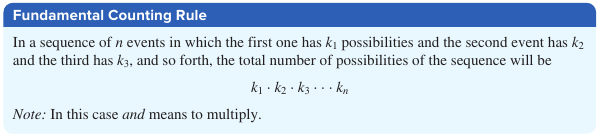
\includegraphics[width=\textwidth]{fcr.png} \pause
		
		Let's look at a few examples.
	\end{frame}

	\begin{frame}{Fundamental Counting Rule}
		A lottery game called Quinto is played by choosing 5 numbers, each from 0 through 9. How many numbers are possible? If repeats were not allowed, how many numbers would be possible? \pause
		
		a) Repetitions allowed: \\
		For the first number, there are 10 options (0-9) \pause
		Since repeats are allowed, there are also 10 options for the second number, and so on. \pause
		
		So there are $10 \cdot 10 \cdot 10 \cdot 10 \cdot 10 = 10^5 = 100,000$ possible numbers. \pause
		
		b) Repetitions not allowed: \\
		There are still 10 possibilities for the first number. \pause
		For the second number, there are 9 possibilities (since we've used one already).
		For the third number, there are 8 possibilities, and so on. \pause
		
		There are $10 \cdot 9 \cdot 8 \cdot 7 \cdot 6 = 30,240$ possible numbers.
	\end{frame}

	\begin{frame}{Fundamental Counting Rule}
		A cell phone company offers 4 different models, each in 6 colors, and each available with any one of 5 calling plans. How many combinations are possible? \pause
		
		There are $4 \cdot 6 \cdot 5 = 120$ combinations. \pause
		
		Given the characters $A, B, C, H, I, T, U, V, 1, 2, 3, 4$, how many seven-character passwords can be made (no repeats are allowed)? \pause
		
		The first character has 12 possibilities. \\ \pause
		The second has 11 possibilities. \\ \pause
		$\vdots$ \\
		The seventh has 6 possibilities. \pause
		
		In total, there are $12 \cdot 11 \cdot 10 \cdot 9 \cdot 8 \cdot 7 \cdot 6 = 3991680$ passwords.
	\end{frame}

	\begin{frame}{Factorial Notation}
		The permuation rule and combination rule each use \textit{factorial notation}. \pause
		
		For any counting number, $n! = n \cdot (n - 1) \cdot (n - 2) \cdot \cdots \cdot 2 \cdot 1$
		
		Example: $7! = 7 \cdot 6 \cdot 5 \cdot 4 \cdot 3 \cdot 2 \cdot 1 = 5040$ \pause
		
		Your graphing calculator has factorial notation built-in.
	\end{frame}

	\begin{frame}{Factorial Notation}
		Use a calculator to compute: \begin{enumerate}[a)]
			\item $11!$
			\item $9!$
			\item $\dfrac{10!}{5!}$ \pause
		\end{enumerate}
		
		a) $39916800$ \pause \\
		b) $362880$ \pause \\
		c) $30240$ 
	\end{frame}

	\begin{frame}{Permutations}
		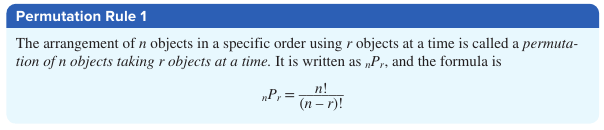
\includegraphics[width=\textwidth]{permutation.png} \pause
		
		The key words here are \textit{in a specific order}. \pause
		
		We use permutations when order matters (e.g. rankings, spellings of words). \pause
		
		Your graphing calculator can compute permutations for you.
	\end{frame}

	\begin{frame}{Permutations}
		Compute: \begin{enumerate}[a)]
			\item $_7 P _5$
			\item $_{26} P _4$
		\end{enumerate}
	
		\onslide<2->{a) \begin{flalign*}
				_7 P _5 &= \dfrac{7!}{(7 - 5)!} & \\
				&= \dfrac{7!}{2!} & \\
				&= 2520
		\end{flalign*}}
		\onslide<3->{b) $358800$}
	\end{frame}

	\begin{frame}{Permutations}
		We can also use permutations when there are identical objects, but this requires a different formula.
		
		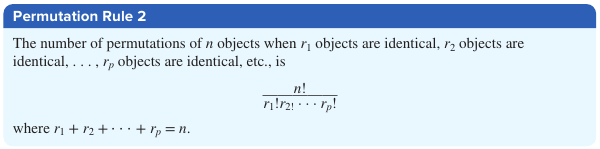
\includegraphics[width=\textwidth]{permutation2.png} \pause
		
		The $_n P _r$ button on your calculator will not work in this case.
	\end{frame}

	\begin{frame}{Permutations}
		To see why having identical objects changes things, consider the word \textit{MISSISSIPPI}. \pause
		
		In particular, let's study ways of arranging the \textit{S}'s in this word. \pause
		
		\textit{MI\red{S}\blue{S}I\orange{S}\violet{S}IPPI} \\
		\textit{MI\violet{S}\orange{S}I\blue{S}\red{S}IPPI} \\
		\textit{MI\blue{S}\violet{S}I\red{S}\orange{S}IPPI} \\
		\textit{MI\orange{S}\blue{S}I\violet{S}\red{S}IPPI} \pause
		
		Using our permutation rule from before, these would each be considered a different permutation. \pause
		
		While each one is indeed a different permutation, you wouldn't be able to tell the difference if I hadn't colored the \textit{S}'s - they're the same word.
	\end{frame}

	\begin{frame}{Permutations}
		How many permutations of the letters can be made from the word \textit{MISSISSIPPI}?
		
		The word \textit{MISSISSIPPI} has 4 \textit{I}'s, 4 \textit{S}'s, 2 \textit{P}'s, and an \textit{M}.
		\begin{flalign*}
			\onslide<3->{\text{Number Permutations} &= \dfrac{11!}{4!4!2!} & \\}
			\onslide<4->{&= 34,650}
		\end{flalign*}
		\onslide<5>{There are a total of 34,650 permutations of the letters}
	\end{frame}

	\begin{frame}{Combinations}
		A \textit{combination} is a selection of distinct objects without regard to order. \pause
		
		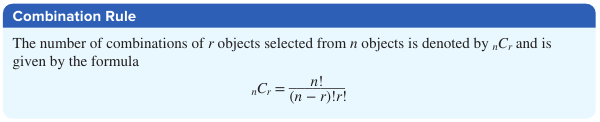
\includegraphics[width=\textwidth]{combination.png} \pause
		
		We use combinations when order doesn't matter. \pause
		
		Your graphing calculator can compute combinations for you.
	\end{frame}

	\begin{frame}{Combinations}
		Compute: \begin{enumerate}[a)]
			\item $_7 C _5$
			\item $_{26} C _4$
		\end{enumerate}
		a) \begin{flalign*}
			\onslide<2->{_7 C _5 &= \dfrac{7!}{(7-5)!5!} & \\}
			\onslide<3->{&= \dfrac{7!}{2!5!} & \\}
			\onslide<4->{&= 21}
		\end{flalign*}
		\onslide<5>{b) $14950$}
	\end{frame}

	\begin{frame}{Practice Problems}
		How many different ways can a city health department inspector visit 5 restaurants in a city with 10 restaurants? \pause
		
		Since we're wanting to take 5 objects from a group of 10 objects, we should use either permutations or combinations. The key question: \textit{does order matter}? \pause
		
		Here, the order in which the inspector visits the restaurants doesn't make any difference. So we should use combinations. \pause
		
		There are $_{10} C _5 = 252$ different ways.
	\end{frame}

	\begin{frame}{Practice Problems}
		In a board of directors composed of 8 people, how many ways can one chief executive officer, one director, and one treasurer be chosen? \pause
		
		We want to choose 3 people from a group of 8, and order matters since each person will have a different job. We should use permutations. \pause
		
		There are $_8 P _3 = 336$ possible ways of assigning the roles.
	\end{frame}

	\begin{frame}{Practice Problems}
		How many different flag signals, each consisting of 7 flags hung vertically, can be made if there are 3 indistinguishable red flags, 2 blue flags, and 2 yellow flags? \pause
		
		This is a permutation problem with identical objects. \pause
		
		There are $\dfrac{7!}{3!2!2!} = 210$ different signals.
	\end{frame}

	\begin{frame}{Practice Problems}
		There are 7 women and 5 men in a department. How many ways can a committee of 4 people be selected, if two of the members must be men and two must be women? \pause
		
		Order doesn't matter here - we should use combinations. \pause
		
		There are 7 women, of which we will select 2. \\
		There are 5 men, of which we will select 2. \pause
		
		So there are $_7 C _2 \cdot _5 C _2 = 10 \cdot 21 = 210$ ways.	
	\end{frame}

	\begin{frame}{Practice Problems}
		There are 7 women and 5 men in a department. How many ways can a committee of 4 people be selected, if at least two of them must be women? \pause
		
		We should still use combinations. This one is a bit trickier since the words at least are used. So there could be 2 women, 3 women, or 4 women on the committee. \pause
		
		We just saw that there are 210 ways of getting a committee with 2 women. \\ \pause
		There are $_7 C _3 \cdot _5 C _1 = 175$ ways of getting 3 women. \\ \pause
		There are $_7 C _4 \cdot _5 C _0 = 35$ ways of getting 4 women. \pause
		
		In total, there are $210 + 175 + 35 = 420$ ways of getting a committee with at least 2 women.
	\end{frame}

	\begin{frame}{Next Steps}
		\begin{itemize}
			\item Read Section 4-5
			\item Watch Video Lesson \#13
			\item Complete Assignment \#6
		\end{itemize}
	
		\vfill
		
		Thanks for watching!
	\end{frame}
	
\end{document}